\section{Questions}
%Each section needs a subsection for the small points on top to show up
\subsection{Dummy}

\begin{frame}{Multifractalité de la chaîne de Fibonacci}
Invariance d'échelle géométrique $\implies$ multifractalité du spectre et des fonctions d'onde

\centering
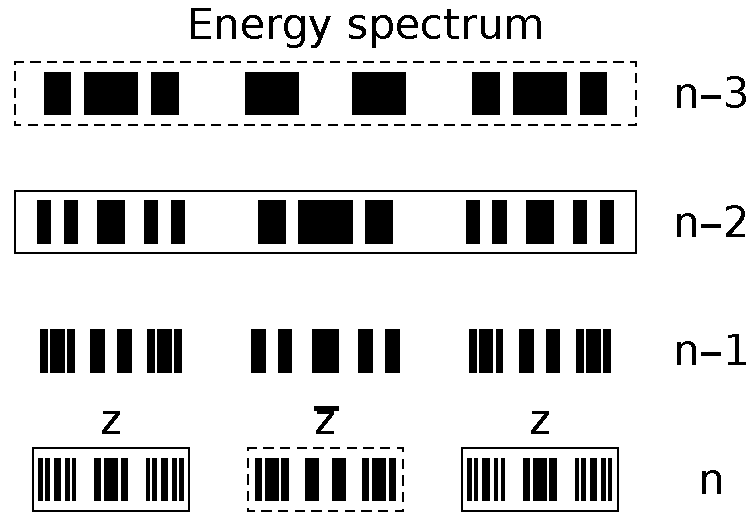
\includegraphics[width=0.5\columnwidth]{img/4_questions/recursive_construction_spectrum}
\end{frame}

\begin{frame}{Multifractalité de la phase localisée à $N$ corps}

\centering
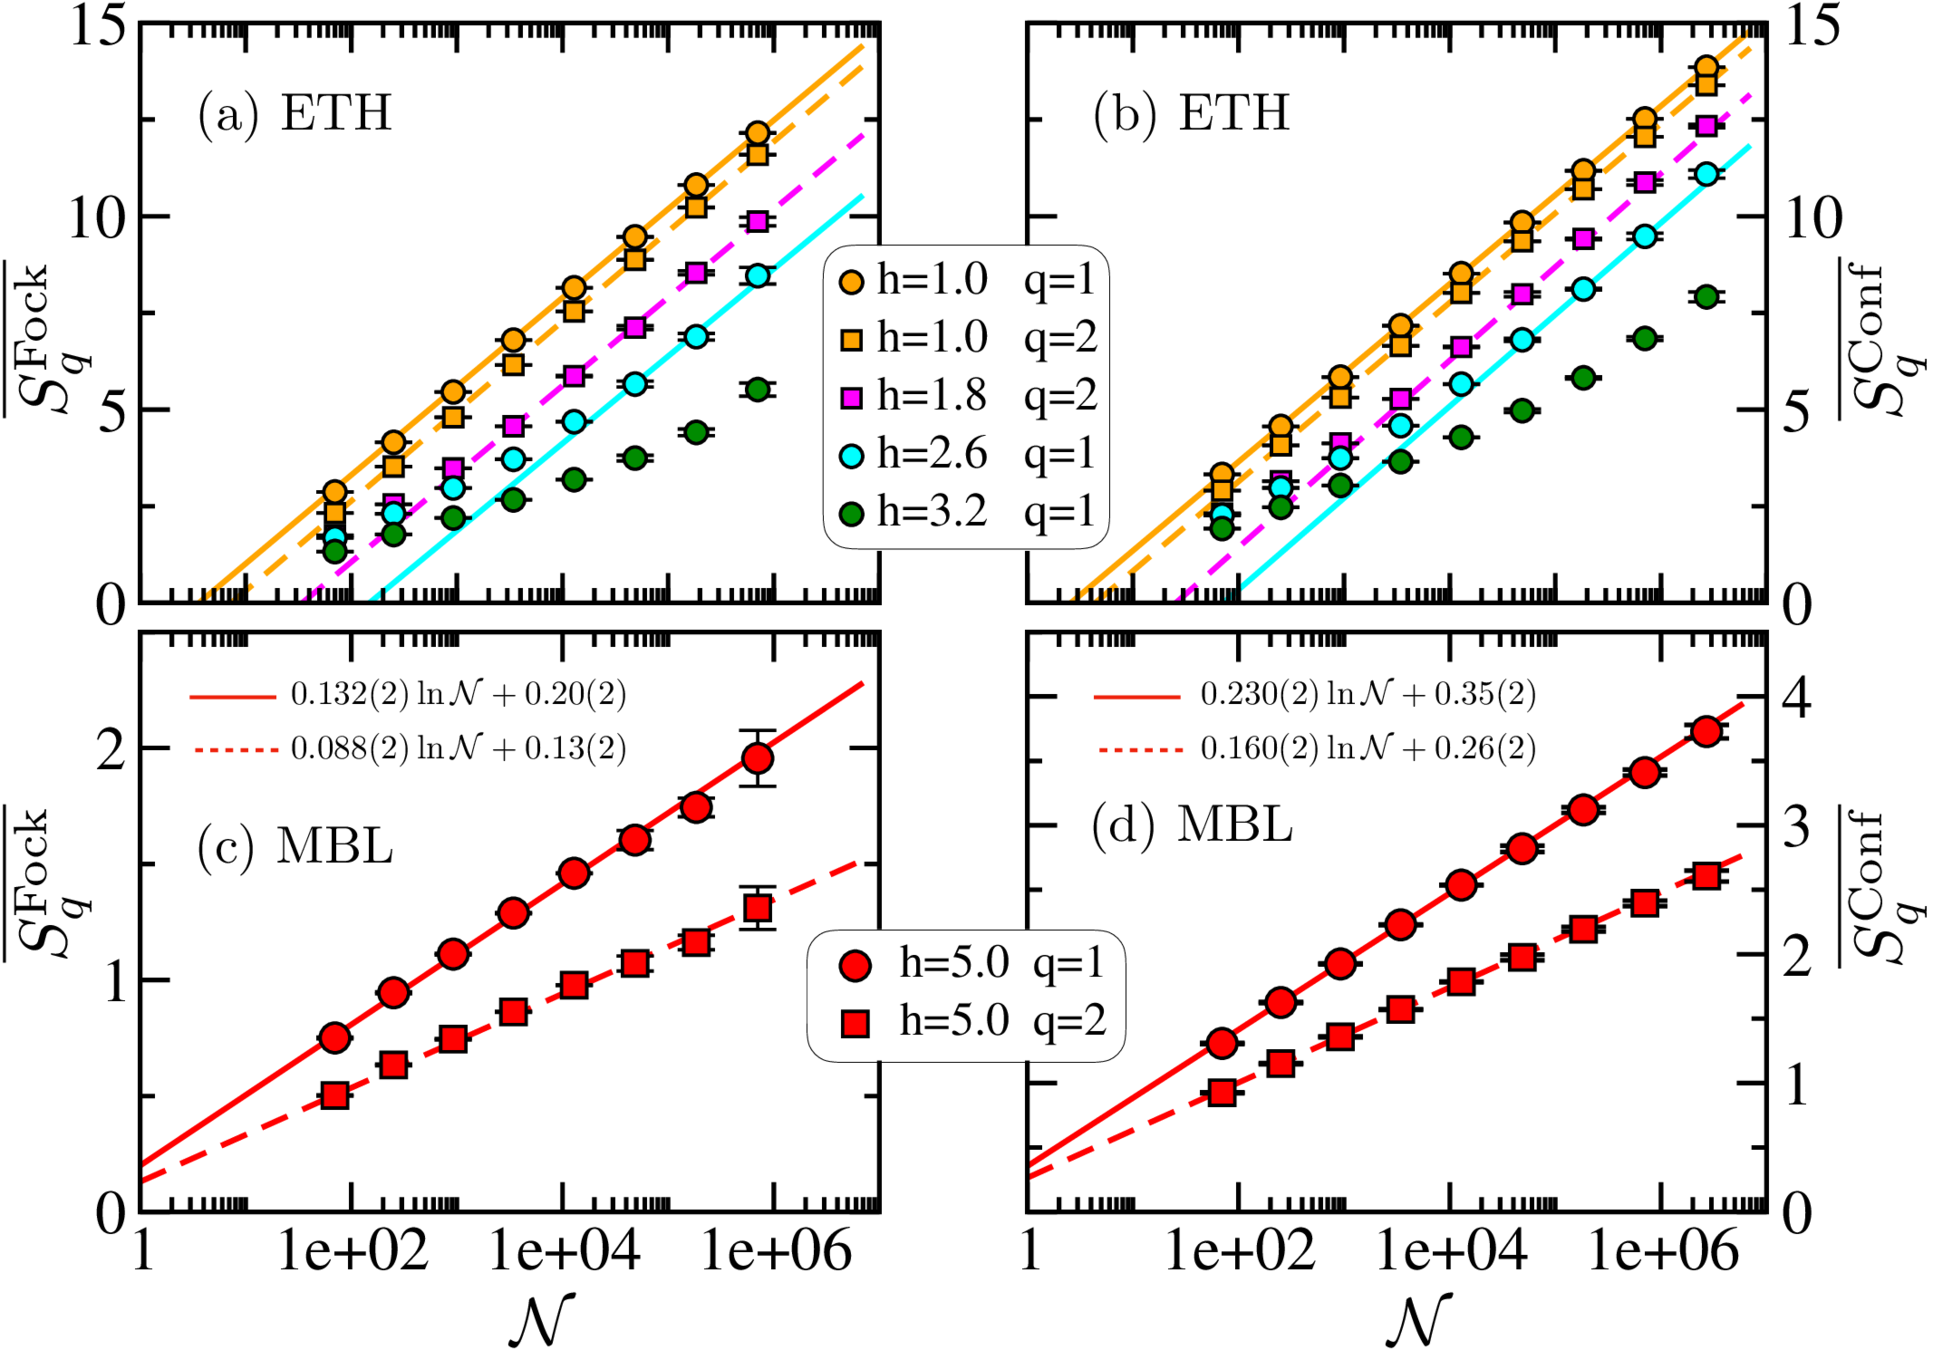
\includegraphics[width=0.4\columnwidth]{img/4_questions/scalings}
%
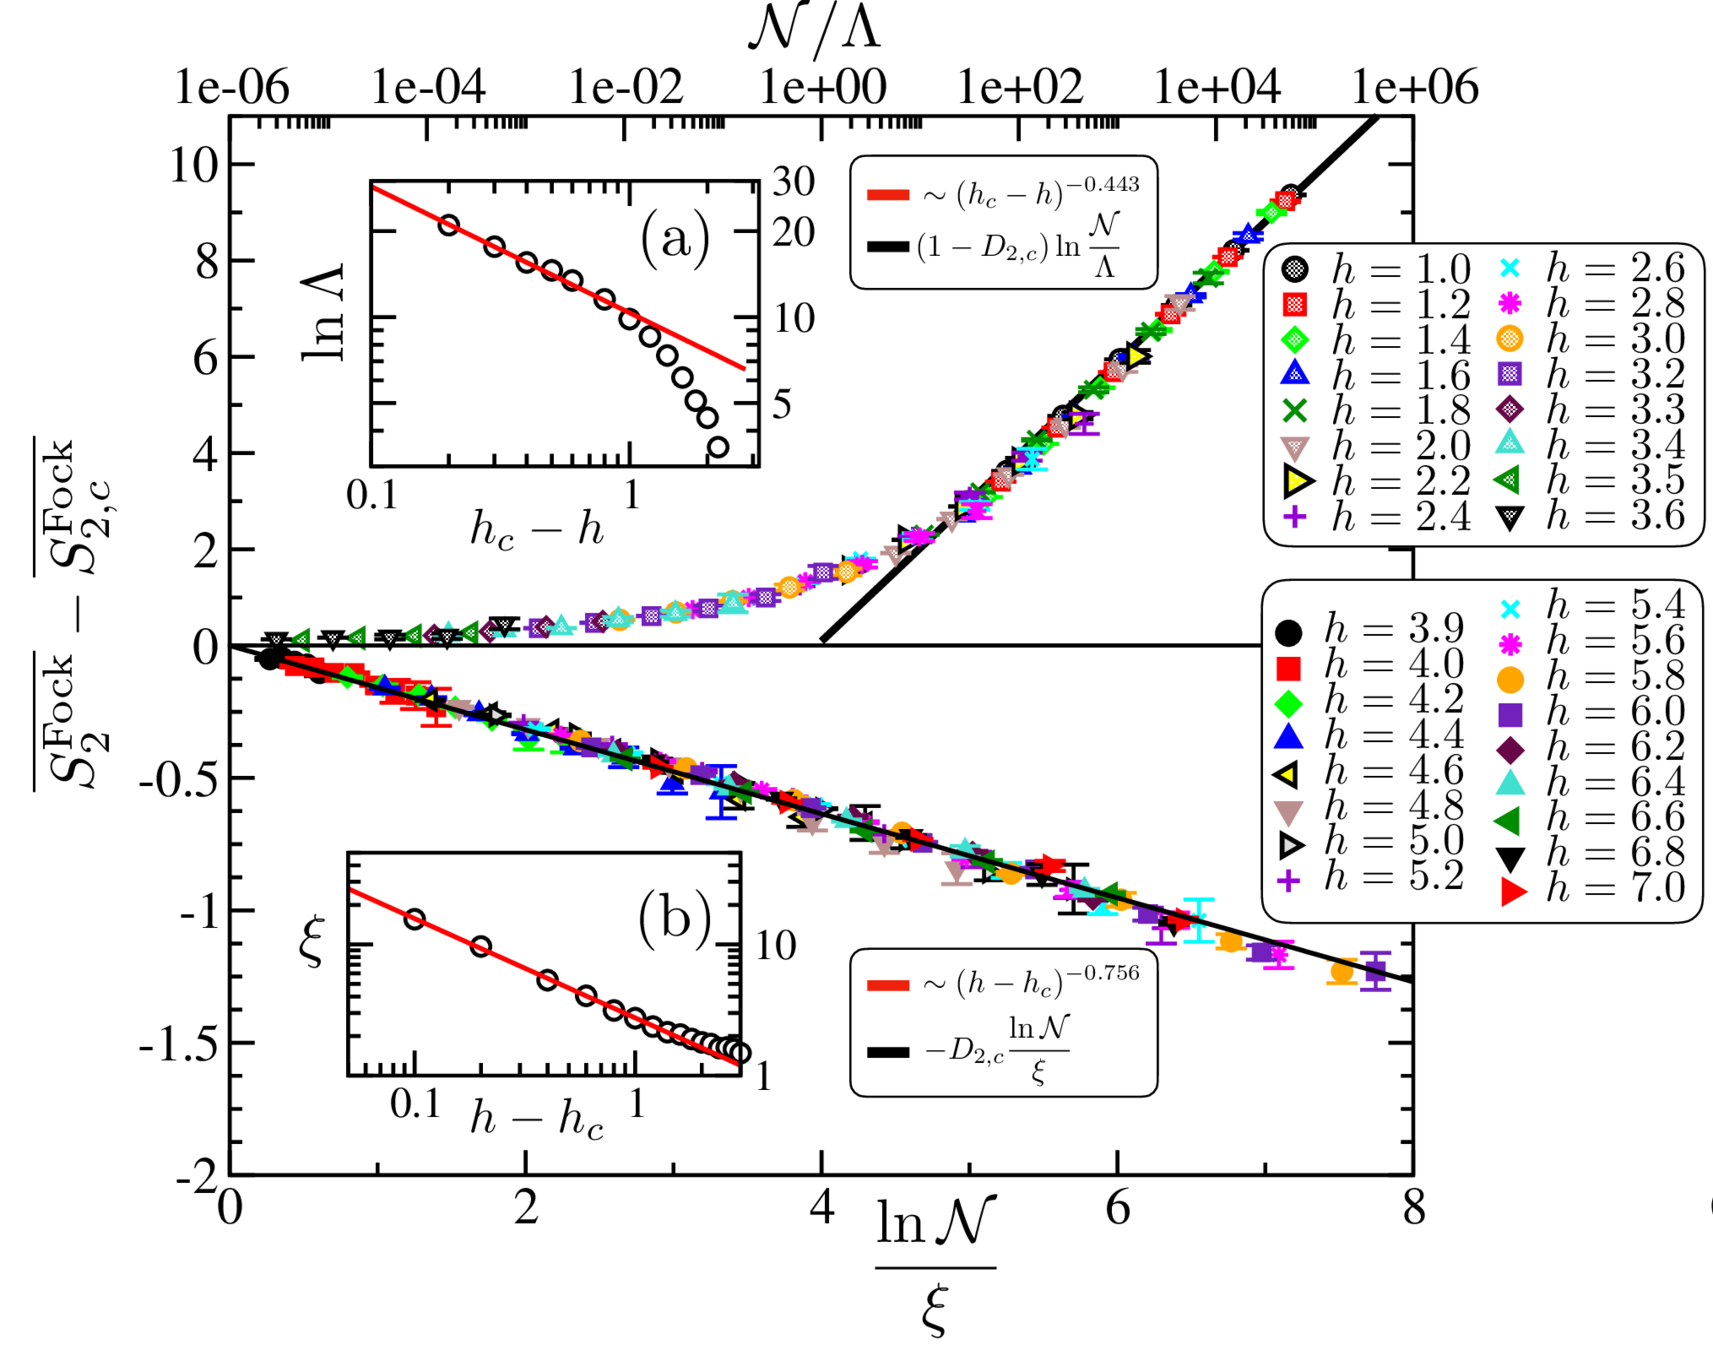
\includegraphics[width=0.4\columnwidth]{img/4_questions/scaling-laws-Fock}

\end{frame}

\begin{frame}{Multifractalité et transitions de phase}
\centering
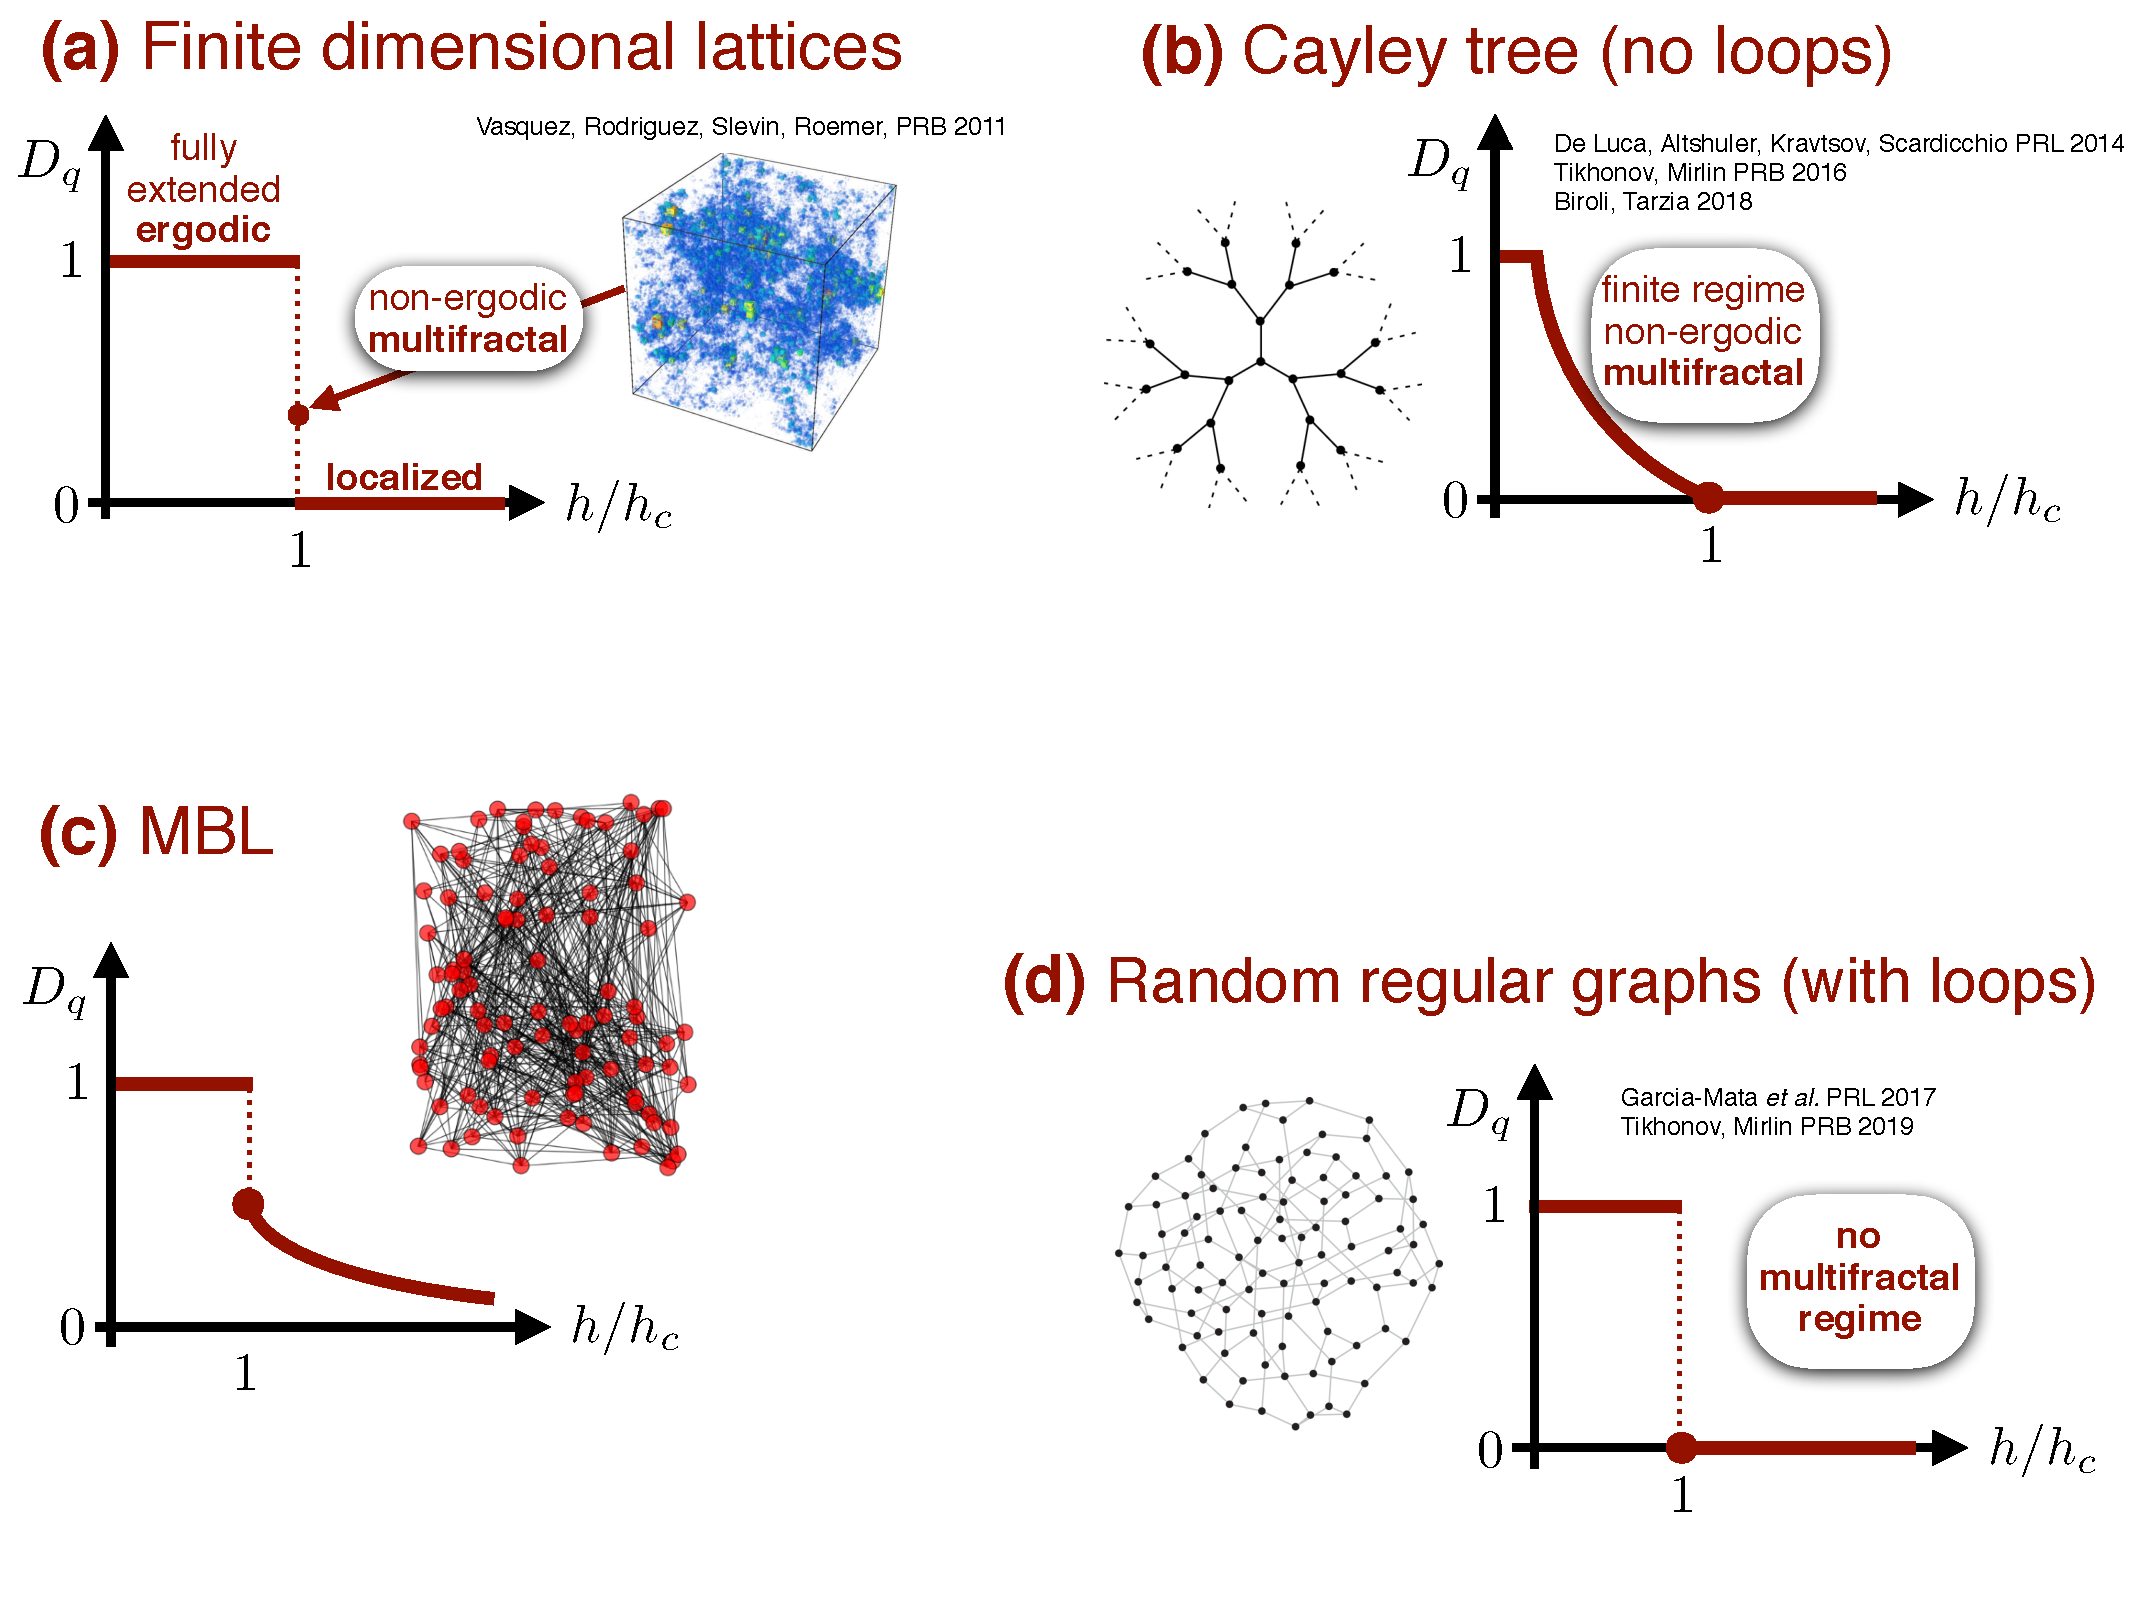
\includegraphics[width=0.6\textwidth]{img/4_questions/Dq}
\end{frame}

\begin{frame}{Blocage de Rydberg et dynamique contrainte}
Nombre quantique principal élevé ($n \geq 50$) $\to$ interactions fortes

Deux atomes :
\[
	H = \Omega( X_1 + X_2) + V Q_1 Q_2
\]
$Q = \frac{1 + Z}{2}$, Van der Waals : $V \propto 1/r^6$.

Régime de blocage de Rydberg : $V \gg \Omega$ $\to \xcancel{\uparrow \uparrow}$
\end{frame}

\begin{frame}{Diagonalisation exacte des circuits quantiques}
Circuits de \textbf{Floquet} : opérateur d'évolution périodique de période $\tau$:
\[
	\ket{\psi(t = n \tau)} = U^n \ket{\psi(0)}
\]
$U$ \textbf{matrice dense} $2^L \times 2^L$ $\implies$ stockage impossible pour $L > 15$.

Circuit quantique 

$\implies$ $U = $ \textbf{opérateur produit de matrices} (MPO) 

$\implies$ opération $y = U x$ rapide et parallélisable en ``matrix free''

$\implies$ diagonalisation exacte (méthode itérative) jusqu'à $L = 20$.

\end{frame}

\begin{frame}{Description hydrodynamique de l'information quantique}
\begin{block}{Modèle microscopique : croissance d'interface}
\centering
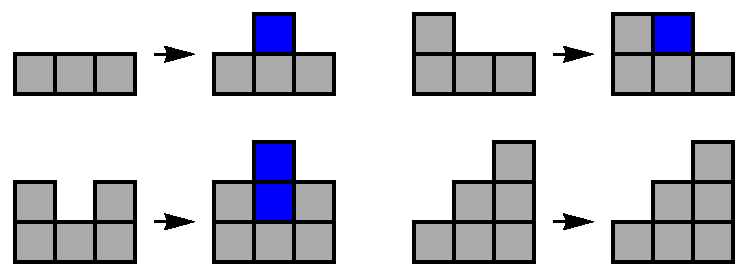
\includegraphics[width=0.4\columnwidth]{img/4_questions/applyingUnitary}

\footnotesize{[Nahum \emph{et al} 17]}
\end{block}
Régime hydrodynamique : KPZ
\[
	\frac{\partial S}{\partial t} = \nu \partial_x^2 S - \frac{\lambda}{2} (\partial_x S)^2 + \eta(x,t) + c
\]

Universalité : exacte pour entropie de Hartley, $d \to \infty$, conjecture : unitaires aléatoires, unitaires de Clifford, chaîne XXZ + environnement \footnotesize{[Nahum \emph{et al} 17, Knap 18]}.
\end{frame}

\begin{frame}{Simulations dans le formalisme de Lindblad}
Flot de Lindblad 
\[
	\frac{d \rho}{d t} = i[\rho, H] + \gamma \sum_k\left( [L_k \rho, L_k^\dagger] + \text{h.c} \right)
\]
Algorithme : 
\begin{enumerate}
	\item Représentation MPO de $\rho$ (troncature éventuelle)
	\item Action du Liouvillien décomposé (Trotter-Suzuki)
\end{enumerate}
Facteur limitant : entropie d'opérateur bornée. Simulation de l'ordre de 100 spins ou qubits.
\end{frame}

\begin{frame}{Atomes froids quasipériodiques}
\centering
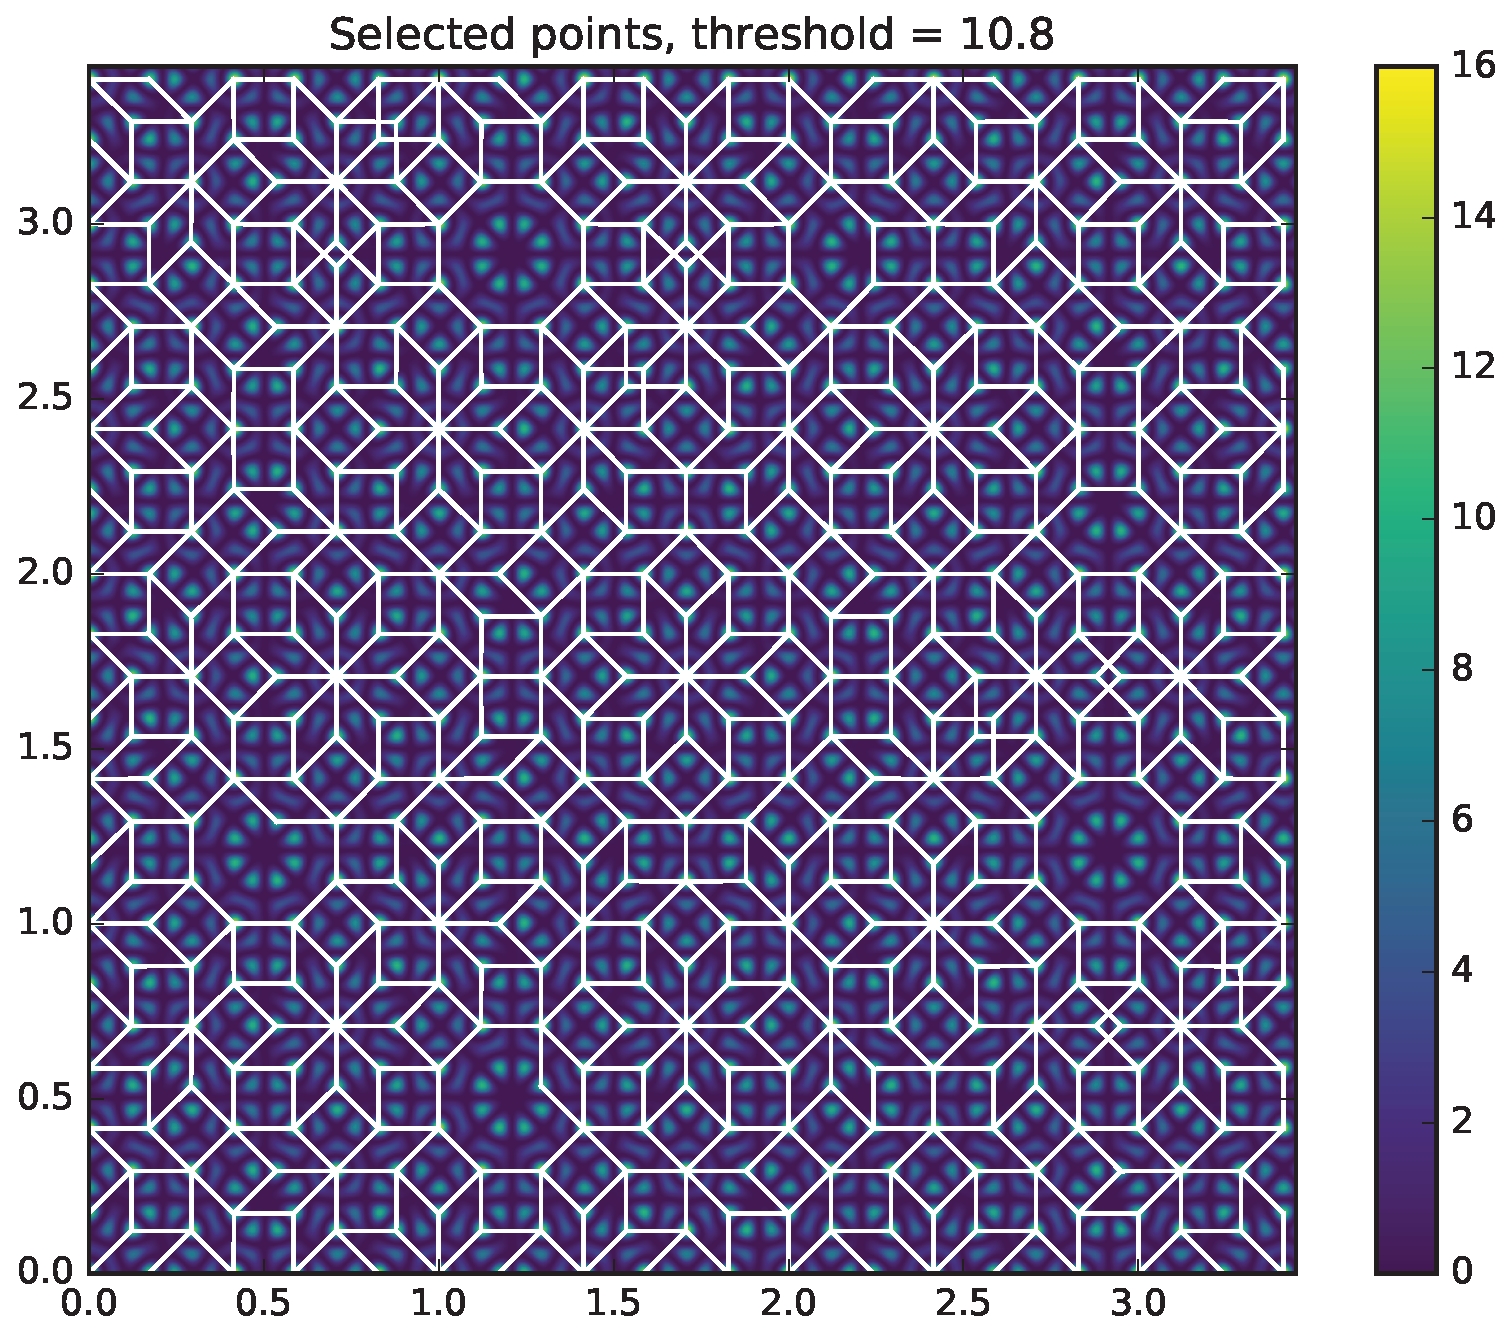
\includegraphics[width=0.5\columnwidth]{img/4_questions/cold_atoms_qc}
\end{frame}

\begin{frame}{Machines thermiques MBL}
Cycle à 4 temps quantique

\begin{columns}
\begin{column}{0.5\textwidth}
\centering
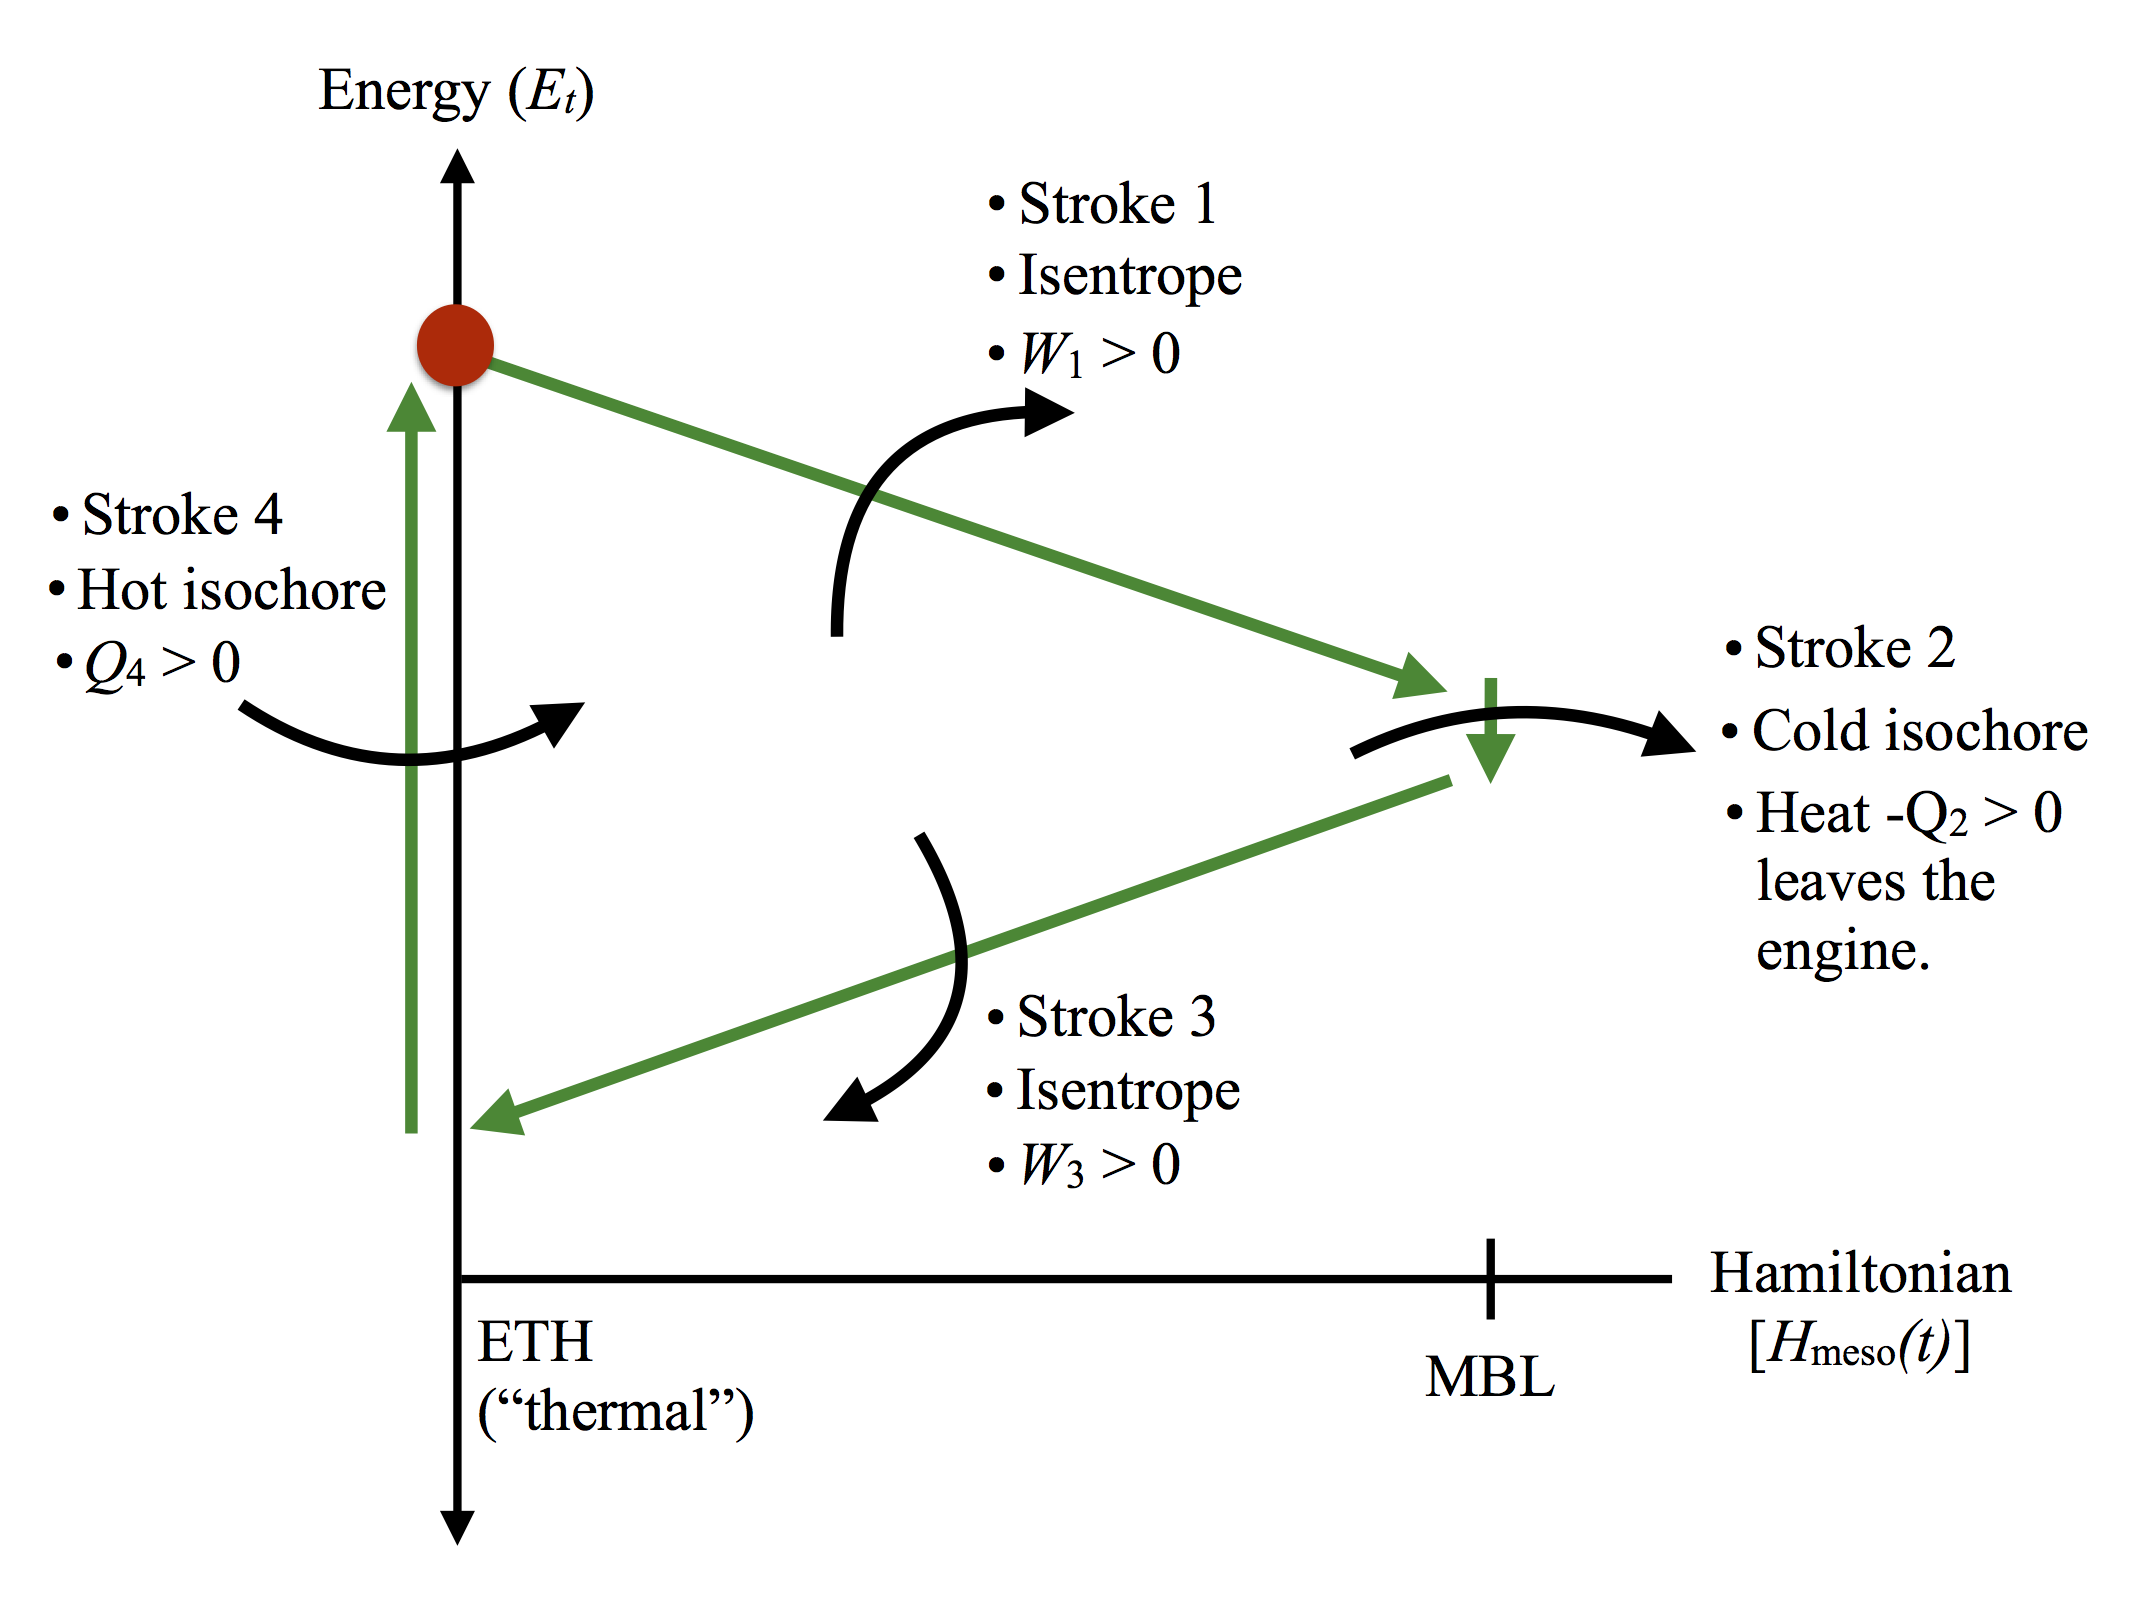
\includegraphics[width=0.8\columnwidth]{img/4_questions/Otto_cycle_MBL}

\footnotesize{[Halpern 18]}
\end{column}
\begin{column}{0.5\textwidth}
\begin{align*}
	\mathcal{P}_v^\text{voiture} &= 1~\text{MW}/\text{m}^3 \\
	\mathcal{P}_v^\text{MBL} &= 100~\text{kW}/\text{m}^3 \\
	\mathcal{P}_v^\text{boîte quantique} &= 1~\text{kW}/\text{m}^3 \\
\end{align*}
\end{column}
\end{columns}
\end{frame}

\begin{frame}{Fidelité et dimensions fractales}
\[
	F(t) = |\braket{\psi(0)}{\psi(t)}|^2
\]
Partant d'un état polarisé en spin,
\[
	F(t\to\infty) = e^{-S_2} = \mathcal{N}^{-D_2}
\]
Imbalance finale d'un état polarisé en spin $\mathcal{C}_0$ :
\[
	I(t \to \infty) = \sum_{k,\mathcal{C}} |\braket{k}{\mathcal{C}}|^2 |\braket{k}{\mathcal{C}_0}|^2 \delta(\mathcal{C}_0, \mathcal{C})
\]
où $-1 \leq \delta(\mathcal{C}_0, \mathcal{C}) \leq 1$ mesure la distance entre les deux configurations.
\end{frame}

\begin{frame}{Bicouches de graphène quasipériodiques}
\centering
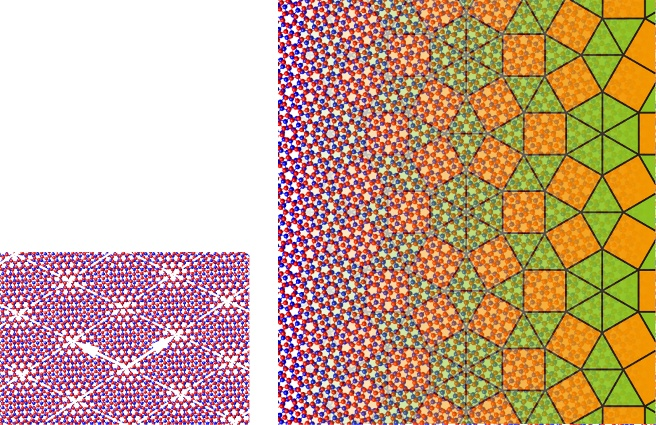
\includegraphics[width=0.5\columnwidth]{img/4_questions/QC_bilayer}

[Yao \emph{et al} 18]
\end{frame}

\begin{frame}{Circuit quantique critique}
\begin{columns}
\begin{column}{0.5\textwidth}
\centering
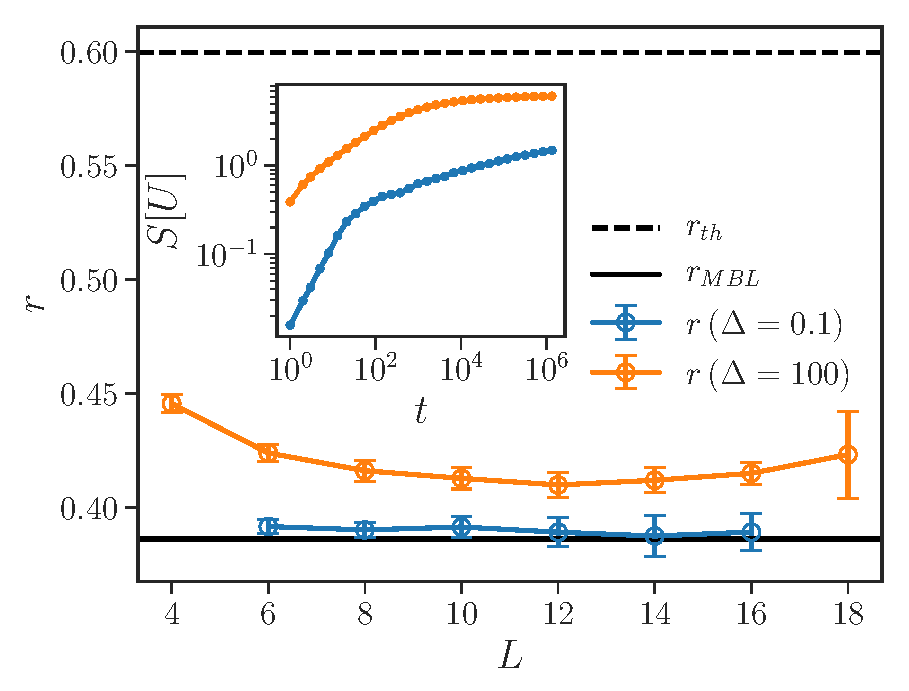
\includegraphics[width=\columnwidth]{img/4_questions/rgaps}
\end{column}
\begin{column}{0.5\textwidth}
\centering
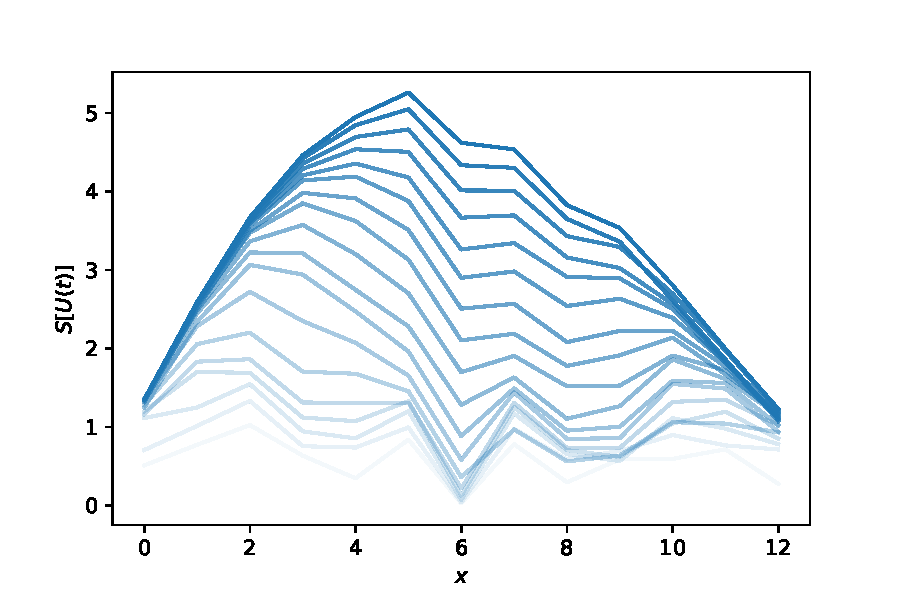
\includegraphics[width=\columnwidth]{img/4_questions/OpEnt_bottlenecks}
\end{column}
\end{columns}
\end{frame}

